\documentclass[12pt]{article}         
\usepackage{fullpage}
\usepackage[shortlabels]{enumitem}
\usepackage{amsmath}
\usepackage{graphicx}

\usepackage{courier} %% Sets font for listing as Courier.
\usepackage{listings, xcolor}
\lstset{
tabsize = 4, %% set tab space width
showstringspaces = false, %% prevent space marking in strings, string is defined as the text that is generally printed directly to the console
numbers = left, %% display line numbers on the left
commentstyle = \color{green}, %% set comment color
keywordstyle = \color{blue}, %% set keyword color
stringstyle = \color{red}, %% set string color
rulecolor = \color{black}, %% set frame color to avoid being affected by text color
basicstyle = \small \ttfamily , %% set listing font and size
breaklines = true, %% enable line breaking
numberstyle = \tiny,
}

%\usepackage{amsmath}
%\usepackage{amssymb}
%\usepackage{enumitem}

\title{250 Homework $\#$4}
\author{Aidan Chin \footnote{Collaborated with Nobody.}}

\begin{document}
\maketitle

\section*{\textbf{P4.7.2} [10 pts]}
Prove by induction on strings that for any binary string $w$, $(oc(w))^R$ = $oc(w^R)$. (See Exercise 4.7.3 for the definition of one’s complement\footnote{If w is a string in $\{0, 1\}^*$, the one’s complement of $w$, $oc(w)$, is the unique string, of the same length as $w$, that has a zero wherever $w$ has a one and vice versa. So, for example, $oc$(101) = 010.}.)

\subsection*{\textbf{Solution:}}
base case:
when $w$ is the empty string, then $w = \lambda$, therefore $\lambda^R \equiv \lambda$ so plugging back in $(oc(\lambda))^R$ = $oc(\lambda)$ and the ones compliment is also the empty string, so they are equivalent \newline
assume a string of length $n$ works $(oc(w))^R$ = $oc(w^R)$\newline
next we need to check when the length is an arbitrary length $n+1$, we can set $w=sd$ where $s$ is a non empty binary string of length $n$ and $d$ is a binary digit 
thus, $oc(w) = oc(s)oc(d)$ and $w^R=d^Rs^R$, now we have all this set up we can plug into the original equation $(oc(w))^R$ = $oc(w^R)$ to get $(oc(s)oc(d))^R$ = $oc(d^Rs^R)$\newline
in the case $d=1$: $(oc(w))^R$ = $oc(w^R)$, $(oc(s)oc(1))^R$ = $oc(1^Rs^R)$ evaluate to get $0(oc(s)^R) = oc(1s^R)$ distribute the last term and we get $oc(1s^R) = 0oc(s^R)$, therefore $0(oc(s)^R) = 0oc(s^R)$ proving our original hypothesis \newline
in the case $d=0$: $(oc(w))^R$ = $oc(w^R)$, $(oc(s)oc(0))^R$ = $oc(0^Rs^R)$ evaluate to get $1(oc(s)^R) = oc(0s^R)$ distribute the last term and we get $oc(0s^R) = 1oc(s^R)$, therefore $1(oc(s)^R) = 1oc(s^R)$ proving our original hypothesis \newline
\newpage
\section*{\textbf{P4.9.8} [10 pts]}
The \textbf{length} of a path in a directed graph is the number of edges in it.

\begin{enumerate}[(a)]
    \item  Give a recursive definition of length, based on the recursive definition of paths in this section.


    \item  Let $\alpha$ be a path from $x$ to $y$, $\beta$ be a path from $y$ to $z$, and $\gamma$ be the path from $x$ to $z$ guaranteed by the Transitivity Theorem of this section. Prove that the length of $\gamma$ is the length of $\alpha$ plus the length of  $\beta$. (Let $\alpha$ be an arbitrary path and use induction on all paths  $\beta$, as in the proof of the Transitivity Theorem.)

\end{enumerate}
\subsection*{\textbf{Solution:}}

\begin{enumerate}[(a)]
    \item 
    \begin{lstlisting}[language = Java , frame = trBL , firstnumber = last , escapeinside={(*@}{@*)}]
    public int length(parentnode)
    {\\returns length of a path
        if(parentnode.child == NULL) return 0;
        return 1 + length(parentnode.child);
    }
    \end{lstlisting}
    \item base case is $\alpha$ is the smallest part of $\gamma$ possible, this is when $\alpha$ has no nodes in it. therefore $\beta$ and $\gamma$ are the same path so they have the same length \newline
    assume when $\alpha$ is an arbitrary length, length($\alpha$) + length($\beta$) = length($\gamma$)\newline
    the definition of a path is the number of edges in the path, therefore if you remove one edge from $\beta$ and add it to $\alpha$ then you still have the same number of edges if added together. so if $\alpha$ concatenated with $\beta=\gamma$ then length($\alpha$) + length($\beta$) = length($\gamma$)
    
\end{enumerate}


\newpage
\section*{\textbf{P4.10.6} [10 pts]}
\textbf{full binary tree} is a rooted binary tree where every internal node has exactly two children and every path from the root to a leaf has the same length.

\begin{enumerate}[(a)]
    \item Give a recursive definition of full binary trees.

    \item  Determine both the number of leaves and the total number of nodes in a full binary tree of depth $n$. Prove your answers using your inductive definition of full binary trees.
    
\end{enumerate}


\subsection*{\textbf{Solution:}}
\begin{enumerate}[(a)]
    \item base case: a node with no children is a full binary tree \newline recursive case: if a binary tree has a root node and both its children are full binary trees, then the binary tree is also a full binary tree

    \item for every node thats not a leaf, there are 2 children, in any depth n, nodes on depth n are leaves. so for every increment of depth, the number of leaves doubles and the total number of nodes increases by 2x the previous number of leaves. 
    \newline the base case: a tree of size depth 0, has 0 nodes and 0 leafs
    \newline for the inductive step, any tree of depth n has $2^n-1$ nodes and $2^{n-1}$ leafs
    \newline for a case where depth = 1, where there is only one node, using our formulas $2^1-1$ nodes and $2^{1-1}$ leafs which is 1 and 1 respectively
    \newline using what we know from before $2^n$ is exactly half of $2^{n+1}$ so this ensures that for each depth level our number of leaves doubles
    \newline now we need to check that the formula works for $n=k+1$ for $2^{n+1}-1$ and $2^{n+1-1}$, for this increment, it is 2 times bigger for each new depth 1 deeper than before, still satisfying what we found before
    
\end{enumerate}

\newpage
\section*{\textbf{P4.11.3} [10 pts]}
 Prove the claim at the end of the section about the Euclidean Algorithm and Fibonacci numbers. Specifically, prove that if positive naturals $a$ and $b$ are each at most $F(n)$, then the Euclidean Algorithm performs at most $n$ - 2 divisions. (You may assume that $n$ $>$ 2.) (It follows from this result that Fibonacci numbers are the worst case, but you may not use that fact to solve this problem!)

\subsection*{\textbf{Solution:}}
base case: $n=3$ we have $f(3) = 2$ if a and b are at most 2 then the Euclidean Algorithm needs 1 division. $2\%2 = 0$
\newline inductive step: assume hypothesis is true.
\newline prove n = k+1 is true 
\newline if $a \le b$ then after the first division, it is reduced to the Euclidean alg for a and ($b\%a$), since $b\%a$ is always going to be less than a, both a and $b\%a$ are going to be at most F(k), by our inductive hypothesis this requires at most k-2 divisions
\newline if $b<a$ then after the first divisions it is reduced to the Euclidean alg for b and $a\%b$ since $a\%b$ is always < b, both b and $a\%b$ are going to be at most F(k), again by our inductions, it will require at most k-2 divisions
\newline for each case, divisions for n=k+1 is at most k-2+1 = k-1, which is n-2

\newpage
\section*{\textbf{P4.11.8} [10 pts]}
 The \textbf{Sierpinski gadget} is defined by a sequence of two-dimensional figures as follows: 
\begin{itemize}
    \item $S_0$ is an equilateral triangle.

    \item Each subsequent $S_i$ is a union of $3^i$ equilateral triangles.

    \item  We make $S_{i+1}$ from $S_i$ by taking each triangle in $S_i$, connecting the midpoints of its three sides to make a smaller triangle, and deleting this smaller triangle from the figure

\end{itemize}
 Figure 4-30 shows the first four figures $S_0, S_1, S_2$, and $S_3$
\begin{figure}[ht]
    \centering
    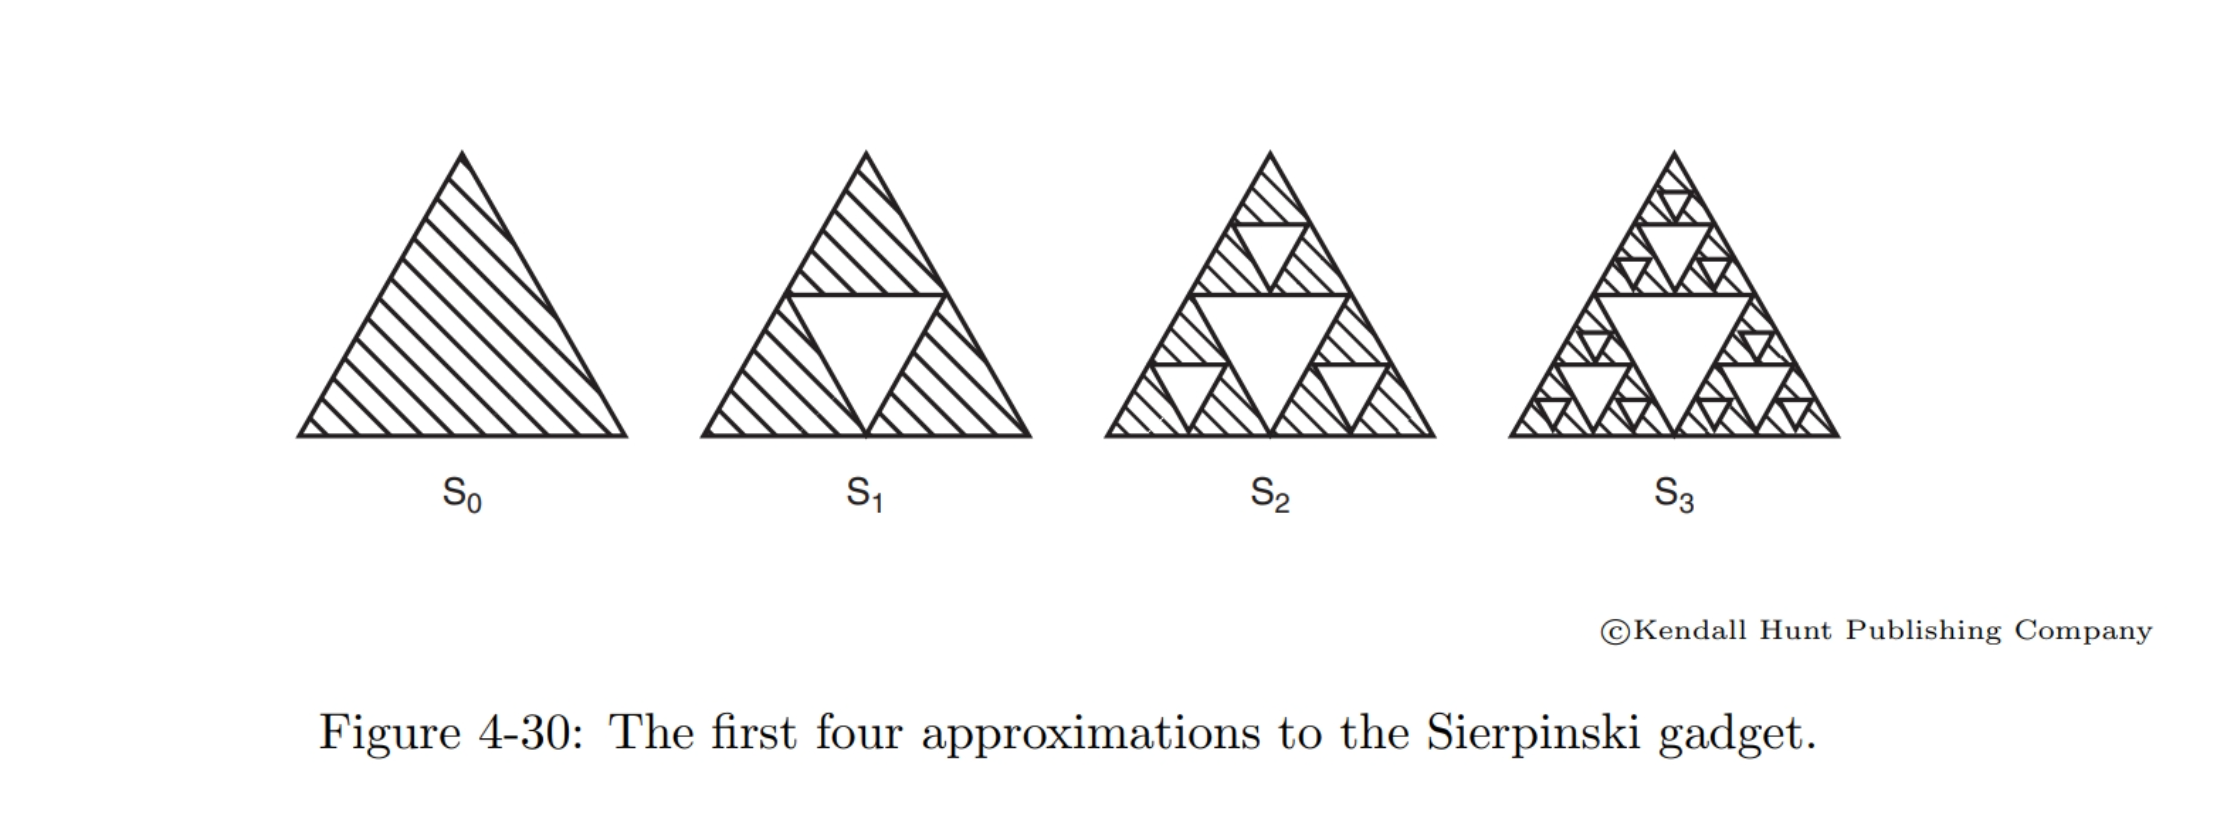
\includegraphics[width=0.75\linewidth]{4-30.png}
\end{figure}
\begin{enumerate}[(a)]
    \item Prove by induction that there are exactly $3^i$ triangles in $S_i$.

    \item Give a formula for the total area of $S_i$ and prove this formula correct by induction
    
\end{enumerate}

\subsection*{\textbf{Solution:}}
\begin{enumerate}[(a)]
    \item 
base case: $S_0$, where the number of triangles is 1, 
\newline inductive step: assume hypothesis is true
\newline prove n=k+1 is true
\newline each iteration splits each triangle into 3 smaller triangles, thus multiplying each level by 3
\newline using this information we find that $3^k$ is some number of triangles and we need to see that $3^{k+1}$ is exactly 3 times more triangles, using what we know about exponents, each increase of 1 in the exponent, multiplies it by the base another time, so $3^{k+1}=3^k*3$, proving our hypothesis
    \item each iteration removes 1/4 of each triangle
\newline inductive step: the area of the gadget is defined by $a*(\frac{1}{4})^n$, where a is area of original equilateral triangle. \newline for each iteration the area is reduced by 1/4
\newline prove n=k+1 is true,
\newline just like before, prove that each step of this formula reduces the area by 1/4 of before. we find that for each iteration in exponents its multiplying the the base again so $a*(\frac{1}{4})^k*\frac{1}{4} \equiv a*(\frac{1}{4})^{k+1}$
\end{enumerate}



\newpage
\section*{\textbf{P9.1.4} [10 pts]}
 Let $G$ be a tree and let $x$ and $y$ be any two nodes such that $(x, y)$ is $not$ an edge. Let $H$ be the graph obtained from $G$ by adding the edge $(x, y)$. Prove that $H$ has exactly one simple cycle.

\subsection*{\textbf{Solution:}}
G has no cycles, but adding the edge $(x,y)$ makes a cycle in the graph H, to prove this we assume that there is another cycle that exists without edge $(x,y)$ but we know that in graph G there is no cycles, so there must be only one new cycle created.

\newpage
\section*{\textbf{P9.3.4} [10 pts]}
 A \textbf{monotone} boolean expression is one with only $\land$ and $\lor$ operators, and no $\lnot$, $\oplus$, $\rightarrow$, or $\leftrightarrow$ operators. Prove by induction on monotone boolean expressions that if every leaf of the expression is \texttt{true}, the value of the expression is \texttt{true}, and similarly for every leaf being \texttt{false}.

\subsection*{\textbf{Solution:}}
using only AND and OR operators\newline
for the most simple monotone expression using both operators, a simple $A\land A \lor A$ can be easily shown because if they are all TRUE or all FALSE, they can be represented by the same thing
\newline if A = TRUE, then the expression is TRUE and if A= FALSE then the expression is FALSE, if we increase the complexity of this monotone expression, we can simply replace one of the $A$ by either $A\land A$ or $A\lor A$
\newline in the case of adding an OR $A\land A \lor (A\lor A)$ we can find that if A is FALSE than the increased part is still FALSE, then we have effectively the original expression, which will still be FALSE and the same for TRUE
\newline in the case of adding an AND $A\land A \lor (A\land A)$ we can find that if A is FALSE than the increased part is still FALSE, then we have effectively the original expression, which will still be FALSE and the same for TRUE


\newpage


\section*{\textbf{P9.4.6} [10 pts]}
 In the \textbf{logic boat puzzle}, you are on one side of a river with a cabbage, a goat, and a wolf, and you want to cross the river with all three items, using a boat which can take only you and one of the items at a time. There is an additional constraint that you may not leave the wolf alone with the goat, or the goat alone with the cabbage. Model the state space of this problem by a graph, with nodes for allowable states and an edge from node $x$ to node $y$ if there is a legal crossing of the boat that changes the state from $x$ to $y$. (Note: You will need to review the solution in the textbook for Exercise 4.11.7.)
\begin{enumerate}[(a)]
    \item Write down the graph representing the state space and explain what each node and edge represents.

    \item Is there a solution to the puzzle?  If there is no solution, prove that there is no solution. If there is a solution, show a solution, step by step.

    \item If your answer in part (b) was that there is no solution, just write “no solution” here.  If your answer to part (b) is that there is a solution now answer ``whether there is more than one solution".  If there is only one solution, explain why the answer in part (b) is the only solution.  If there is more than one solution, describe the second solution.
    
\end{enumerate}

\subsection*{\textbf{Solution:}}
\begin{enumerate}[(a)]
    \item Each node represents a state, and each arrow represents a valid transition from one state to another from left to right SSSS equals cabbage, goat, wolf, boat on the start side, DDDD means all on the destination side
    \begin{figure}[ht]
        \centering
        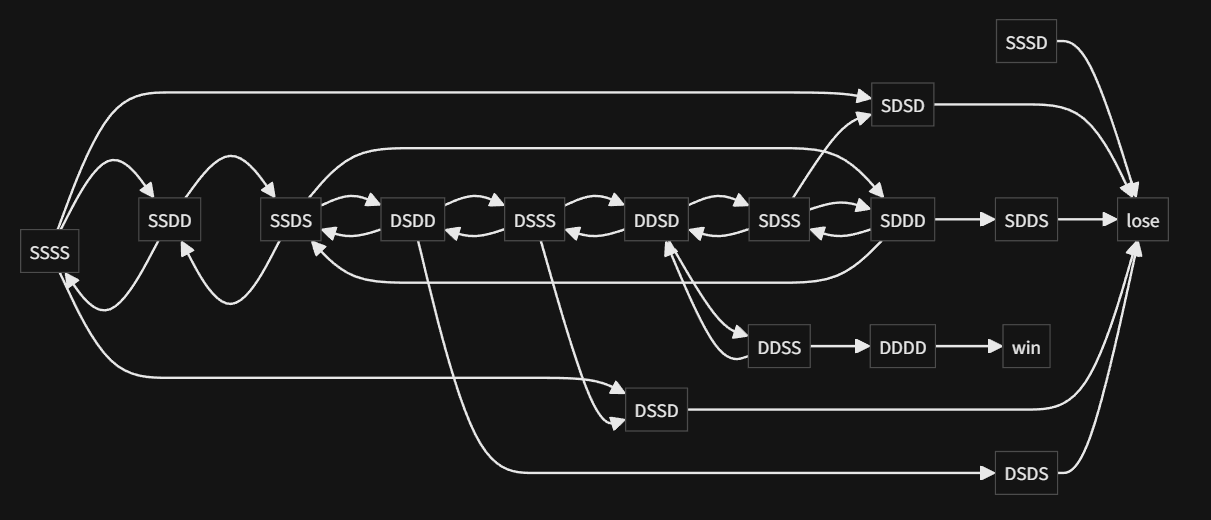
\includegraphics[width=0.75\linewidth]{4-6.png}
    \end{figure}
    \item yes the solution is to take the goat first, then the wolf, swapping the goat with the wolf and bringing them back to the other side, then taking the cabbage and swapping the goat, finally going back for the goat.

    \item no there is not more than one solution, unless you include loops in the graph, because there is only one way to the end without backtracking
    
\end{enumerate}


\newpage
\section*{\textbf{P9.8.7} [10 pts]}
 Figure 9-15 shows a weighted undirected graph representing driving distances among eight cities in the northeastern United States. Carry out a uniform-cost search to find the shortest-path distance $to$ Boston from each city $x$.
\begin{figure}[ht]
    \centering
    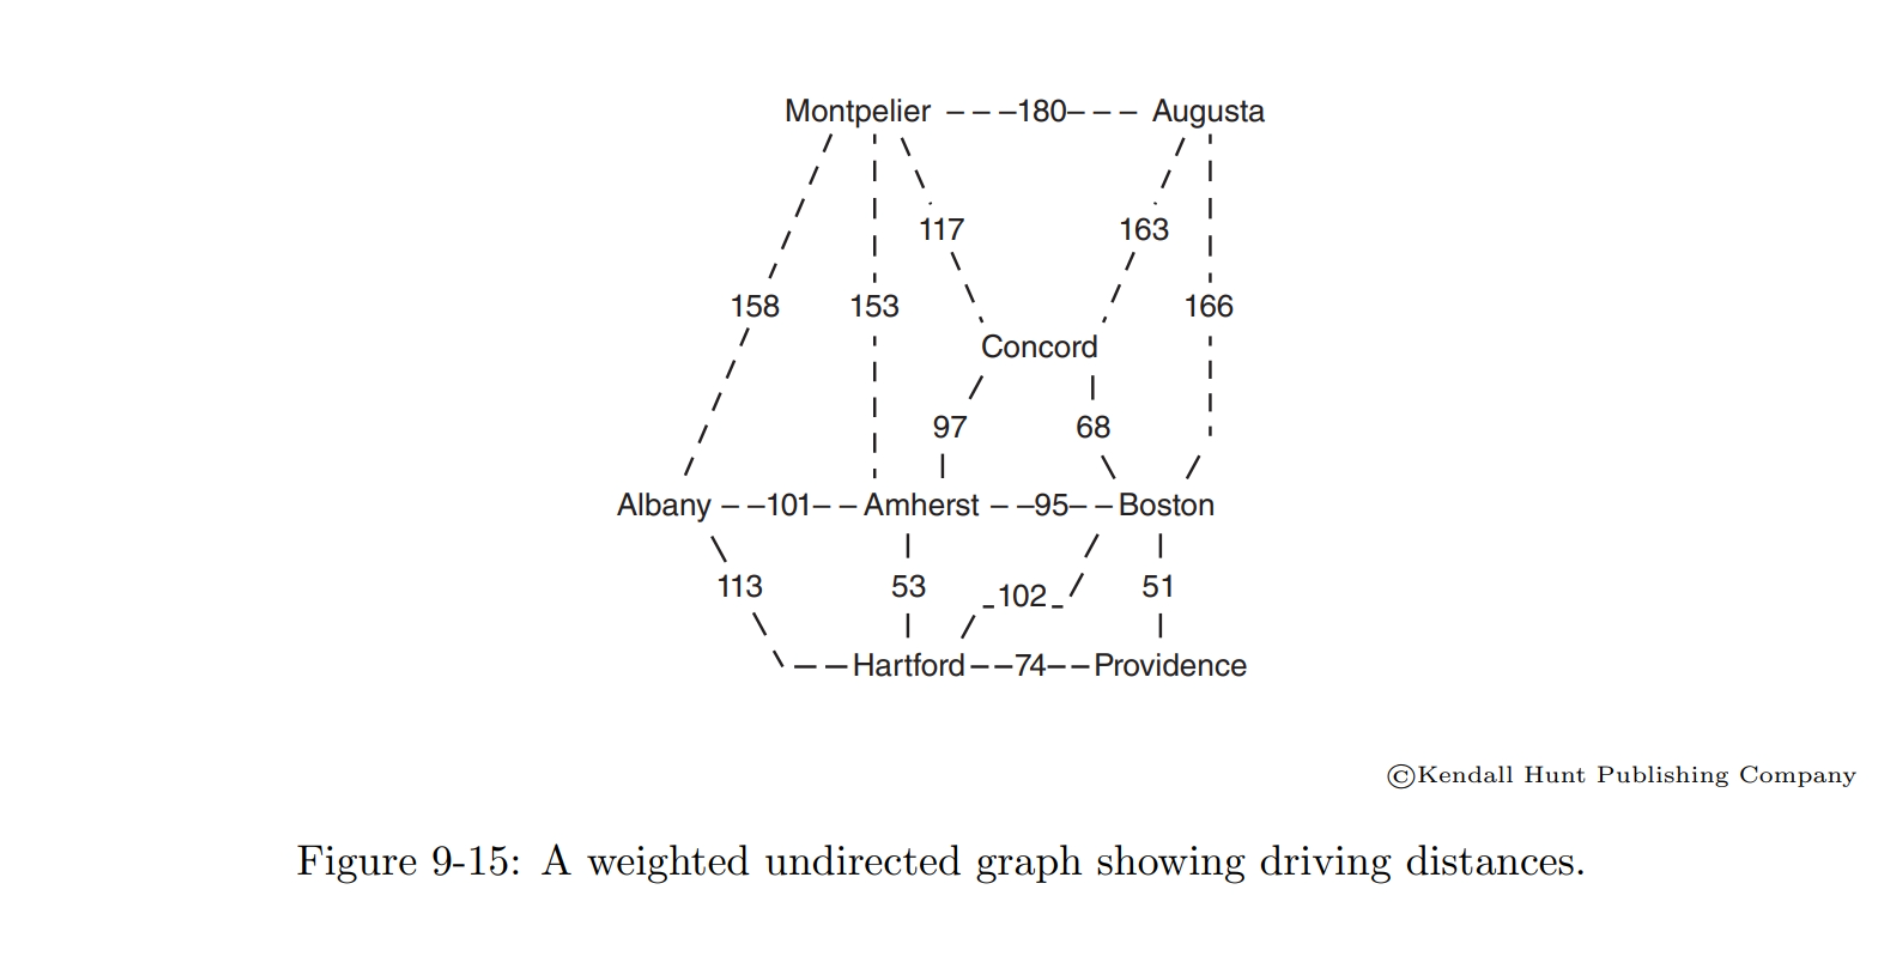
\includegraphics[width=0.75\linewidth]{9-15.png}
\end{figure}

\subsection*{\textbf{Solution:}}

from boston work backwards to find to find providence the closest city and concord the second closest with amherst next, hartfort is close with its shortest path being direct and same with augusta. for the further cities its quickest to get to montpelier through concord and albany through amherst
to do this i found the closest city to boston, providence then compared from providence to each city plus distance to boston, i did this for each city and found the shortest paths to all cities
\newpage
\section*{\textbf{P9.9.1} [10 pts]}
 For the $n$ = 4 version of the Manhattan one-way street graph of Problem 9.8.3\footnote{ Let $M_n$ be a labeled directed graph as follows, modeling a portion of Manhattan Island and its one-way street system. The nodes of $M_n$ are given by pairs of naturals $(i, j)$, with $i \leq n$ and $j \leq n$. There are edges:
 \begin{itemize}
     \item From $(i, j)$ to $(i + 1, j)$ (east), whenever $j$ is even and $i < n$,

     \item From $(i, j)$ to $(i + 1, j)$ (east), whenever $j$ is even and $i < n$,

     \item From $(i, j)$ to $(i, j + 1)$ (north), whenever $i$ is even and $j < n$, 

     \item From $(i, j)$ to $(i, j - 1)$ (south), whenever $i$ is odd and $j > 0$.
     
 \end{itemize}
 Note that (0, 0) is a source node. Assume that the weight of each north-south edge is 1 and that the weight of each east-west edge is 3 (reflecting the fact that east-west blocks are longer in Manhattan).}, with edge weights 1 and 3, conduct a uniform-cost search with $s$ = (1, 1) and $t$ = (3, 3). Then conduct an $A^*$ search for the same start and goal node with $h(i, j)$ equal to the $pedestrian$ distance from $(i, j)$ to (3, 3). (Pedestrians ignore one-way streets, so they can travel edges $or$ $their$ $reversals$ using the given weights.)

\subsection*{\textbf{Solution:}}
conducting the search conduct djikstras, just like the previous problem, search from the closest nodes making your way out to the furthest noting down what paths are the shortest. the shortest path from 1,1 to 3,3 is length 12, one of these paths are 1,1 1,2 2,2 2,3 3,3
\newline doing an A* search is setting the distance to the start node to 0 and all others to infinity, then we explore down the nodes marking down the new distances, we start at the start node, and make our way through the closest nodes until we find something 
\begin{table}[h]
    \centering
    \caption{Node Distance}
    \begin{tabular}{|c|c|}
    \hline
    Node & Distance \\
    \hline
    (1,1) & 0 \\
    (1,2) & 3 \\
    (2,1) & 3 \\
    (1,3) & 6 \\
    (2,2) & 6 \\
    (3,1) & 6 \\
    (1,4) & 9 \\
    (2,3) & 9 \\
    (3,2) & 9 \\
    (4,1) & 9 \\
    (2,4) & 12 \\
    (3,3) & 12 \\
    \hline
    \end{tabular}
    \label{tab:node_distance}
\end{table}

\begin{table}[h]
    \centering
    \caption{Node Distance}
    \begin{tabular}{|c|c|c|c|}
    \hline
    Node & g & h & f \\
    \hline
    (1,1) & 0 & 6 & 6 \\
    (1,2) & 3 & 5 & 8 \\
    (2,1) & 3 & 4 & 7 \\
    (2,2) & 6 & 3 & 9 \\
    (1,3) & 6 & 4 & 10 \\
    (3,1) & 6 & 3 & 9 \\
    (2,3) & 9 & 2 & 11 \\
    \hline
    \end{tabular}
    \label{tab:node_distance}
\end{table}
\newpage
\section*{\textbf{EC: P4.11.9} [10 pts]}
 Following Exercise 4.11.7, we can consider the number $f(n)$ of perfect matchings in a $3 \times 2n$ grid graph, which is the same as the number of ways to tile a $3 \times 2n$ rectangle with $1 \times 2$ dominoes. (Note: You will need to review the solution in the textbook for Exercise 4.11.7.)
 
\begin{enumerate}[(a)]

    \item Prove that $f(0)$ = 1, $f(1)$ = 3, and that for positive $n$, $f(n)$ = 3$f(n - 1)$ + 2$f(n - 2)$ + \ldots + 2$f(0)$.

    \item Prove (probably using the formula in (a)) that for $n >$ 1, $f(n)$ = 4$f(n - 1)$ - $f(n - 2)$. 

    \item Prove by induction (probably using the formula in (b)) that for all naturals $n$, $f(n)$ = $((1 + 1/\sqrt{3})(2 + \sqrt{3})^n) + (1 - 1/\sqrt{3})(2 - \sqrt{3})^n))/2$. 

    \item Using any of these formulas, find $f(n)$ for all $n$ with $n \leq$ 5.
    
\end{enumerate}

\subsection*{\textbf{Solution:}}

\begin{enumerate}[(a)]

    \item base case: f(0) = 1 and f(1) = 3\newline
    inductive step: assume f(n-1) and f(n-2) are true
    \newline prove: consider 3 by n graph, remove the last column to get a 3 by n-1 graph, then there are f(n-1) perfect matchings
    \newline removing 2 does the same, 3 by n-2 graph with f(n-2) perfect pairs
    in any of these perfect matchings, the vertex in the last column must be matched to one in the first 2 so there are f(n-1)+f(n-2) perfect matchings
    \newline there are also perfect matchings in the 3 by n grid that dont match the vertex in the last column to make this we chose any 2 unmatched vertices in the first columns and match them together, then we can match the remaining to give us 2f(0) perfect matchings
    \newline so the total number of perfect matchings is f(n-1)+f(n-2)+f(0)

    \item we can just substitute in the get 4f(n-1)-f(n-2):
    \newline f(n) = 3f(n-1)+f(n-2)... +2f(0)
=3[3f(n-2)f(n-3)+ ·· +2f(0)]f(n-2)
=9f(n-2)f(n-3)+ .· +6f(0)f(n-2)
=11f(n-2)gf(n-3)+.+6f(0)

    \item sing the formula from part. The formula holds for \( n = 0 \), since \( f(0) = 1 = \frac{{(1 + \frac{1}{\sqrt{3}})(2 + \sqrt{3})^0 + (1 - \frac{1}{\sqrt{3}})(2 - \sqrt{3})^0}}{2} \). Now, suppose that the formula holds for some integer \( n \). We can use this to show that the formula also holds for \( n + 1 \).

    For the case \( n + 1 \), we have:

    \[
    \begin{aligned}
    &f(n + 1) = 4f(n)f(n - 1) \\
    &= 4\left(\frac{{(1 + \frac{1}{\sqrt{3}})(2 + \sqrt{3})^n + (1 - \frac{1}{\sqrt{3}})(2 - \sqrt{3})^n}}{2}\right) \left(\frac{{(1 + \frac{1}{\sqrt{3}})(2 + \sqrt{3})^{n - 1} + (1 - \frac{1}{\sqrt{3}})(2 - \sqrt{3})^{n - 1}}}{2}\right) \\
    &= \frac{{\left((1 + \frac{1}{\sqrt{3}})(2 + \sqrt{3})^n + (1 - \frac{1}{\sqrt{3}})(2 - \sqrt{3})^n\right)}}{2} \times \frac{{\left((1 + \frac{1}{\sqrt{3}})(2 + \sqrt{3})^{n - 1} + (1 - \frac{1}{\sqrt{3}})(2 - \sqrt{3})^{n - 1}\right)}}{2} \\
    &= \frac{{(1 + \frac{1}{\sqrt{3}})(2 + \sqrt{3})^n \times \left((1 + \frac{1}{\sqrt{3}})(2 + \sqrt{3})^{n - 1} + (1 - \frac{1}{\sqrt{3}})(2 - \sqrt{3})^{n - 1}\right)}}{4} \\
    &\quad + \frac{{(1 - \frac{1}{\sqrt{3}})(2 - \sqrt{3})^n \times \left((1 + \frac{1}{\sqrt{3}})(2 + \sqrt{3})^{n - 1} + (1 - \frac{1}{\sqrt{3}})(2 - \sqrt{3})^{n - 1}\right)}}{4}. \\
    &= \frac{{(1 + \frac{1}{\sqrt{3}})(2 + \sqrt{3})^{n + 1} + (1 - \frac{1}{\sqrt{3}})(2 - \sqrt{3})^{n + 1}}}{2}.
    \end{aligned}
    \]
    
    Thus, by induction, the formula holds for all natural numbers \( n \).
    \item 
    To find \( f(n) \) for all \( n < 5 \), plug in to compute the values for each \( n \).

\[
\begin{aligned}
f(0) &= \frac{{(1 + \frac{1}{\sqrt{3}})(2 + \sqrt{3})^0 + (1 - \frac{1}{\sqrt{3}})(2 - \sqrt{3})^0}}{2} = 1 \\
f(1) &= \frac{{(1 + \frac{1}{\sqrt{3}})(2 + \sqrt{3})^1 + (1 - \frac{1}{\sqrt{3}})(2 - \sqrt{3})^1}}{2} = 3 \\
f(2) &= \frac{{(1 + \frac{1}{\sqrt{3}})(2 + \sqrt{3})^2 + (1 - \frac{1}{\sqrt{3}})(2 - \sqrt{3})^2}}{2} = 7 \\
f(3) &= \frac{{(1 + \frac{1}{\sqrt{3}})(2 + \sqrt{3})^3 + (1 - \frac{1}{\sqrt{3}})(2 - \sqrt{3})^3}}{2} = 15 \\
f(4) &= \frac{{(1 + \frac{1}{\sqrt{3}})(2 + \sqrt{3})^4 + (1 - \frac{1}{\sqrt{3}})(2 - \sqrt{3})^4}}{2} = 31
\end{aligned}
\]

\( f(n) \) for all \( n < 5 \) is given by the sequence \( 1, 3, 7, 15, 31 \).

\end{enumerate}

\end{document} 